\section{Context: Physical Computing}
\label{sec:domain}

As discussed in the Introduction, the micro:bit is a device
with similarities to the Arduino family of printed 
circuit boards. Such devices as known by the term
{\em physical computing}, as they are designed to be placed in and
interact with our physical environment (as opposed to computer programs
whose main manifestation is realized on a monitor, like games).  
Physical computing lives in the spaces between computing and many other disciplines:
art, industrial design, health, environmental monitoring; it has
close ties to cyber-physical systems, embedded systems, and IoT. 


% from https://www.nsf.gov/news/special_reports/cyber-physical/
% "Cyber-physical systems integrate sensing, computation, 
% control and networking into physical objects and infrastructure, 
% connecting them to the Internet and to each other."
%
% https://en.wikipedia.org/wiki/Embedded_system

Physical computing benefits:
\begin{itemize}
\item broad reach because of diverse applications of physical computing -- leverage fine arts, music, design, etc. in projects;
\item increased motivation and connections because of tangible visible outcome (rather than virtual on screen);
\item learning by doing: many ways to achieve goal (no single correct solution)
\item natural division of labor for more complex projects (design, hardware, software, ...)
\item full system view of computing: hardware and software working together.
\end{itemize}

\subsection{Wiring and Arduino}

% from thesis of Hernando Barragán:
% - http://people.interactionivrea.org/h.barragan/thesis/thesis_low_res.pdf 
% - Wiring: Prototyping Physical Interaction Design
% - June 2004

% http://wiring.org.co/

% https://globenewswire.com/news-release/2017/05/19/988294/0/en/Arduino-Welcomes-Hernando-Barrag%C3%A1n-as-Arduino-Chief-Design-Architect.html

To help explain the BBC micro:bit, it's very instructive to understand
Hernando Barragan's 2003 Master's thesis, ``Wiring: Prototyping Physical Interaction Design'',
the inspiration for the Arduino system~\cite{Barragan}. His objective was to make it easier
for non-technical creators, such as artists and designers, to leverage
electronics in their their work by simplifying the hardware and programming
experience. In particular, he said of existing work:
``Current prototyping tools for electronics and programming are mostly targeted 
to engineering, robotics and technical audiences.''  
Of Wiring's design, he identified the following key concepts:
\begin{itemize}
\item a simple cross-platform integrated development environment (IDE) to create so-called ``sketches'';
\item simplified application programming interfaces (APIs) to access a microcontroller's resources;
\item leverage open source compiler/linker toolchain, transparent to the end user;
\item a bootloader to make it easy to upload a compiled sketch to the microcontroller;
\end{itemize}
Also key to Wiring  was openness of both the hardware and software
comprising the system.

But, still some issues:
\begin{itemize}
    \item reliance on the C language and C compiler (needs to be installed)
    \item very poor experience in IDE
    \item USB bootloader requires device drivers on some systems 
\end{itemize}

% Uno: (which measures 5.34cm x 6.86cm),

\begin{figure} 
    \begin{tabular}{cc}
      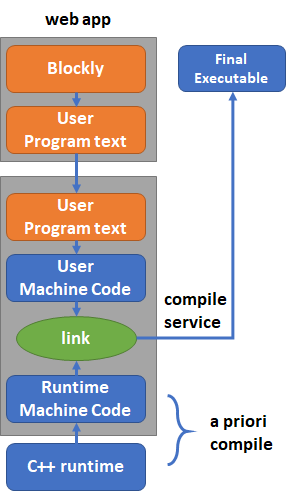
\includegraphics[width=1.5in]{images/bbc.png} & 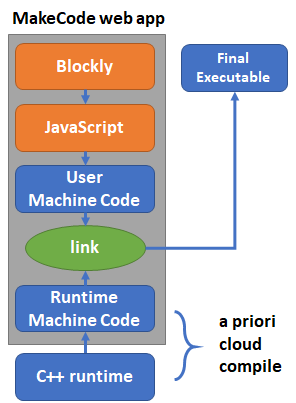
\includegraphics[width=1.5in]{images/makecode.png} \\
        (a) & (b) 
    \end{tabular}
    \caption{\label{fig:design}Web and compiler designs: (a) initial BBC design; (b) final design, as implemented in MakeCode.}
    \end{figure}

    
\subsection{The BBC micro:bit}

BBC micro:bit inherits the raw PCB nature of Arduino 
(everything is visible to the end user).

First key idea of the BBC micro:bit: NO WIRING REQUIRED!
Second key idea: smaller.
Third key idea: web app for programming and simulating.

As shown in Figure~\ref{fig:design}(a), in the BBC design
the text of a user's program (whether derived from Blockly or produced directly by the user)
is submitted to a compile service that returns a final executable to be copied onto a micro:bit (connected to the host 
computer by USB) via a specialized loader application.  

avoiding the need for a compile service for user code (as shown 
in Figure~\ref{fig:design}(b));